%%%%%%%%%%%%%%
%% Run LaTeX on this file several times to get Table of Contents,
%% cross-references, and citations.

%% If you have font problems, you may edit the w-bookps.sty file
%% to customize the font names to match those on your system.

%% w-bksamp.tex. Current Version: Feb 16, 2012
%%%%%%%%%%%%%%%%%%%%%%%%%%%%%%%%%%%%%%%%%%%%%%%%%%%%%%%%%%%%%%%%
%
%  Sample file for
%  Wiley Book Style, Design No.: SD 001B, 7x10
%  Wiley Book Style, Design No.: SD 004B, 6x9
%
%
%  Prepared by Amy Hendrickson, TeXnology Inc.
%  http://www.texnology.com
%%%%%%%%%%%%%%%%%%%%%%%%%%%%%%%%%%%%%%%%%%%%%%%%%%%%%%%%%%%%%%%%

%%%%%%%%%%%%%
% 7x10
%\documentclass{wileySev}

% 6x9
\documentclass{wileysix}

\usepackage{graphicx}
\usepackage{listings}

\usepackage{color}
 
\definecolor{codegreen}{rgb}{0,0.6,0}
\definecolor{codegray}{rgb}{0.5,0.5,0.5}
\definecolor{codepurple}{rgb}{0.58,0,0.82}
\definecolor{backcolour}{rgb}{0.95,0.95,0.92}
 
\lstdefinestyle{mystyle}{
    backgroundcolor=\color{backcolour},   
    commentstyle=\color{codegreen},
    keywordstyle=\color{magenta},
    numberstyle=\tiny\color{codegray},
    stringstyle=\color{codepurple},
    basicstyle=\footnotesize,
    breakatwhitespace=false,         
    breaklines=true,                 
    captionpos=b,                    
    keepspaces=true,                 
    numbers=left,                    
    numbersep=5pt,                  
    showspaces=false,                
    showstringspaces=false,
    showtabs=false,                  
    tabsize=2,
    language=sh
}
 
\lstset{style=mystyle}

%%%%%%%
%% for times math: However, this package disables bold math (!)
%% \mathbf{x} will still work, but you will not have bold math
%% in section heads or chapter titles. If you don't use math
%% in those environments, mathptmx might be a good choice.

% \usepackage{mathptmx}

% For PostScript text
\usepackage{w-bookps}

%%%%%%%%%%%%%%%%%%%%%%%%%%%%%%%%%%%%%%%%%%%%%%%%%%%%%%%%%%%%%%%%
%% Other packages you might want to use:

% for chapter bibliography made with BibTeX
% \usepackage{chapterbib}

% for multiple indices
% \usepackage{multind}

% for answers to problems
% \usepackage{answers}

%%%%%%%%%%%%%%%%%%%%%%%%%%%%%%
%% Change options here if you want:
%%
%% How many levels of section head would you like numbered?
%% 0= no section numbers, 1= section, 2= subsection, 3= subsubsection
%%==>>
\setcounter{secnumdepth}{3}

%% How many levels of section head would you like to appear in the
%% Table of Contents?
%% 0= chapter titles, 1= section titles, 2= subsection titles, 
%% 3= subsubsection titles.
%%==>>
\setcounter{tocdepth}{2}

%% Cropmarks? good for final page makeup
%% \docropmarks

%%%%%%%%%%%%%%%%%%%%%%%%%%%%%%
%
% DRAFT
%
% Uncomment to get double spacing between lines, current date and time
% printed at bottom of page.
% \draft
% (If you want to keep tables from becoming double spaced also uncomment
% this):
% \renewcommand{\arraystretch}{0.6}
%%%%%%%%%%%%%%%%%%%%%%%%%%%%%%

%%%%%%% Demo of section head containing sample macro:
%% To get a macro to expand correctly in a section head, with upper and
%% lower case math, put the definition and set the box 
%% before \begin{document}, so that when it appears in the 
%% table of contents it will also work:

\newcommand{\VT}[1]{\ensuremath{{V_{T#1}}}}

%% use a box to expand the macro before we put it into the section head:

\newbox\sectsavebox
\setbox\sectsavebox=\hbox{\boldmath\VT{xyz}}

%%%%%%%%%%%%%%%%% End Demo


\begin{document}


\booktitle{IMPLEMENTASI GENETIK ALGORITMA MENGGUNAKAN CODEIGNITER}
\subtitle{Dalam 24 Jam}

\authors{Rolly M. Awangga\\
\affil{Informatics Research Center}
%Floyd J. Fowler, Jr.\\
%\affil{University of New Mexico}
}

\offprintinfo{PETUNJUK PENINGKATAN KOMPETENSI , First Edition}{Rolly M. Awangga}

%% Can use \\ if title, and edition are too wide, ie,
%% \offprintinfo{Survey Methodology,\\ Second Edition}{Robert M. Groves}

%%%%%%%%%%%%%%%%%%%%%%%%%%%%%%
%% 
\halftitlepage

\titlepage


\begin{copyrightpage}{2019}
%Survey Methodology / Robert M. Groves . . . [et al.].
%\       p. cm.---(Wiley series in survey methodology)
%\    ``Wiley-Interscience."
%\    Includes bibliographical references and index.
%\    ISBN 0-471-48348-6 (pbk.)
%\    1. Surveys---Methodology.  2. Social 
%\  sciences---Research---Statistical methods.  I. Groves, Robert M.  II. %
%Series.\\
%
%HA31.2.S873 2007
%001.4'33---dc22                                             2004044064
\end{copyrightpage}

\dedication{`Jika Kamu tidak dapat menahan lelahnya belajar, 
Maka kamu harus sanggup menahan perihnya Kebodohan.'
~Imam Syafi'i~}

\begin{contributors}
\name{Rolly Maulana Awangga,} Informatics Research Center., Politeknik Pos Indonesia, Bandung,
Indonesia



\end{contributors}

\contentsinbrief
\tableofcontents
\listoffigures
\listoftables
\lstlistoflistings


\begin{foreword}
Sepatah kata dari Kaprodi, Kabag Kemahasiswaan dan Mahasiswa
\end{foreword}

\begin{preface}
Buku ini diciptakan bagi yang awam dengan git sekalipun.

\prefaceauthor{R. M. Awangga}
\where{Bandung, Jawa Barat\\
Februari, 2019}
\end{preface}


\begin{acknowledgments}
Terima kasih atas semua masukan dari para mahasiswa agar bisa membuat buku ini 
lebih baik dan lebih mudah dimengerti.

Terima kasih ini juga ditujukan khusus untuk team IRC yang 
telah fokus untuk belajar dan memahami bagaimana buku ini mendampingi proses 
Intership.
\authorinitials{R. M. A.}
\end{acknowledgments}

\begin{acronyms}
\acro{ACGIH}{American Conference of Governmental Industrial Hygienists}
\acro{AEC}{Atomic Energy Commission}
\acro{OSHA}{Occupational Health and Safety Commission}
\acro{SAMA}{Scientific Apparatus Makers Association}
\end{acronyms}

\begin{glossary}
\term{git}Merupakan manajemen sumber kode yang dibuat oleh linus torvald.

\term{bash}Merupakan bahasa sistem operasi berbasiskan *NIX.

\term{linux}Sistem operasi berbasis sumber kode terbuka yang dibuat oleh Linus Torvald
\end{glossary}

\begin{symbols}
\term{A}Amplitude

\term{\hbox{\&}}Propositional logic symbol 

\term{a}Filter Coefficient

\bigskip

\term{\mathcal{B}}Number of Beats
\end{symbols}

\begin{introduction}

%% optional, but if you want to list author:

\introauthor{Rolly Maulana Awangga, S.T., M.T.}
{Informatics Research Center\\
Bandung, Jawa Barat, Indonesia}

Pada era disruptif  \index{disruptif}\index{disruptif!modern} 
saat ini. git merupakan sebuah kebutuhan dalam sebuah organisasi pengembangan perangkat lunak.
Buku ini diharapkan bisa menjadi penghantar para programmer, analis, IT Operation dan Project Manajer.
Dalam melakukan implementasi git pada diri dan organisasinya.

Rumusnya cuman sebagai contoh aja biar keren\cite{awangga2018sampeu}.

\begin{equation}
ABC {\cal DEF} \alpha\beta\Gamma\Delta\sum^{abc}_{def}
\end{equation}

\end{introduction}

%%%%%%%%%%%%%%%%%%Isi Buku_


\chapter{XAMPP}
Xampp merupakan singkatan dari X (empat sistem operasi apapun), Apache, Mysql, PHP, dan Perl. Xampp adalah tool yang menyediakan paket perangkat lunak dalam satu buah paket. Dalam paket Xampp sudah terdapat Apache (web server), Mysql (database), PHP (server side scripting), Perl ,FTP server, PhpMyAdmin dan berbagai pustaka bantu lainya. XAMPP adalah perangkat lunak bebas, yang mendukung banyak sistem operasi, merupakan kompilasi dari beberapa program \cite{sugiarto2019aplikasi}.

\section{Tutorial Install Xampp}
\begin{enumerate}
    \item Download terlebih dahulu aplikasi Xampp di https://www.apachefriends.org/index.html, download sesuai sistem operasi yang anda gunakan, pada tutorial kali ini saya akan melakukan instalasi XAMPP di Windows 10.
    
	\item Setelah download aplikasi, lakukan instalasi XAMPP, dengan cara klik kanan pada file instalasi kemudian pilih Open.
		\begin{figure}[!htbp]
    		\centering
    		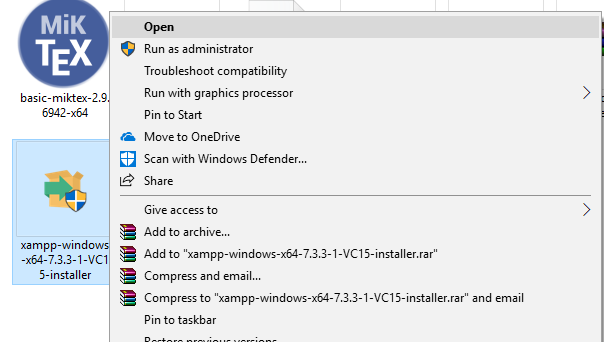
\includegraphics[width=0.5\textwidth]{figures/Xampp2.png}
    		\label{Xampp2}
		\end{figure}
		
	\item Jika pada saat melakukan instalasi muncul peringatan yang bertujuan untuk memastikan apakah Anda akan menginstal aplikasi ini, Silakan klik Ok/Yes untuk melanjutkan instalasi.
		\begin{figure}[!htbp]
    		\centering
    		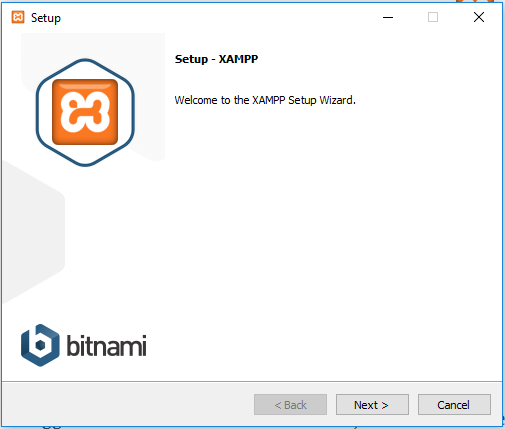
\includegraphics[width=0.5\textwidth]{figures/Xampp3.PNG}
    		\label{Xampp3}
		\end{figure}
		
	\item Klik next untuk melanjutkan, kemudian akan tampil pilihan aplikasi apa yang akan Anda install dan tidak ingin Anda install.
		\begin{figure}[!htbp]
    		\centering
    		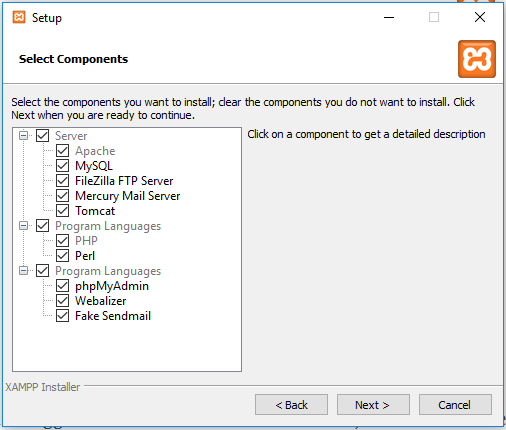
\includegraphics[width=0.5\textwidth]{figures/Xampp4.PNG}
    		\label{Xampp4}
		\end{figure}
		
	\item Tahap selanjutnya adalah memilih folder dimana lokasi instalasi xampp akan disimpan.
		\begin{figure}[!htbp]
    		\centering
    		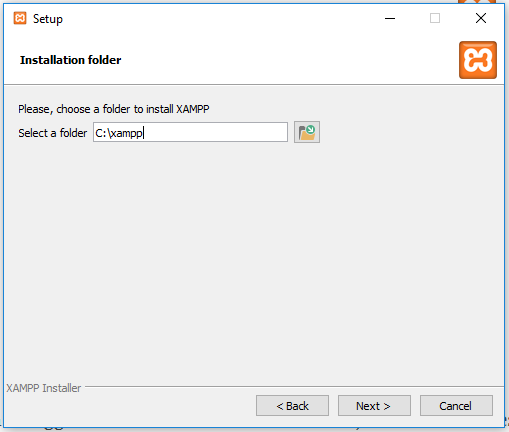
\includegraphics[width=0.5\textwidth]{figures/Xampp5.PNG}
    		\label{Xampp5}
		\end{figure}
		
	\item Silakan hilangkan centang pada “Learn more about Bitnami for XAMPP”, kemudian klik Next.
		\begin{figure}[!htbp]
    		\centering
    		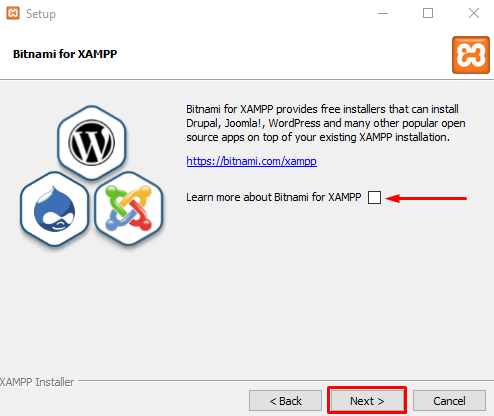
\includegraphics[width=0.5\textwidth]{figures/Xampp6.png}
    		\label{Xampp6}
		\end{figure}
		
	\item Klik next untuk malnjutkan ke proses instalasi xampp.
		\begin{figure}[!htbp]
    		\centering
    		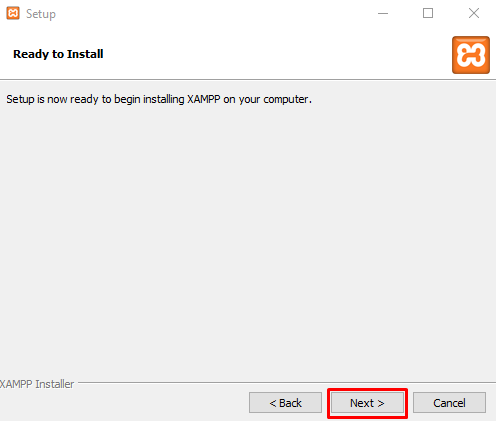
\includegraphics[width=0.5\textwidth]{figures/Xampp7.png}
    		\label{Xampp7}
		\end{figure}
		
	\item Apabila aplikasi sudah terinstal maka akan tampil pertanyaan mengenai apakah Anda ingin langsung menjalankan control panel. Pastikan pilihan tersebut sudah tercentang, kemudian klik tombol Finish.
		\begin{figure}[!htbp]
    		\centering
    		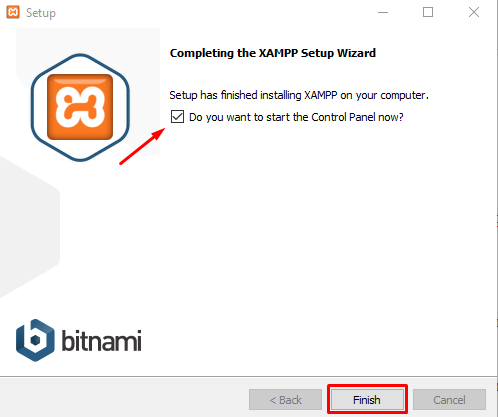
\includegraphics[width=0.5\textwidth]{figures/Xampp8.png}
    		\label{Xampp8}
		\end{figure}
		
	\item Control panel akan muncul otomatis, tapi jika Anda tidak mencentang pilihan di halaman sebelumnya, maka Anda perlu membuka langsung control panel melalui start menu atau folder XAMPP di komputer Anda.
	
	\item Apabila control panel sudah muncul dan terlihat seperti gambar \ref{Xampp9}, maka proses instalasi Xampp berhasil.
		\begin{figure}[!htbp]
    		\centering
    		\caption{Control Panel Xampp}
    		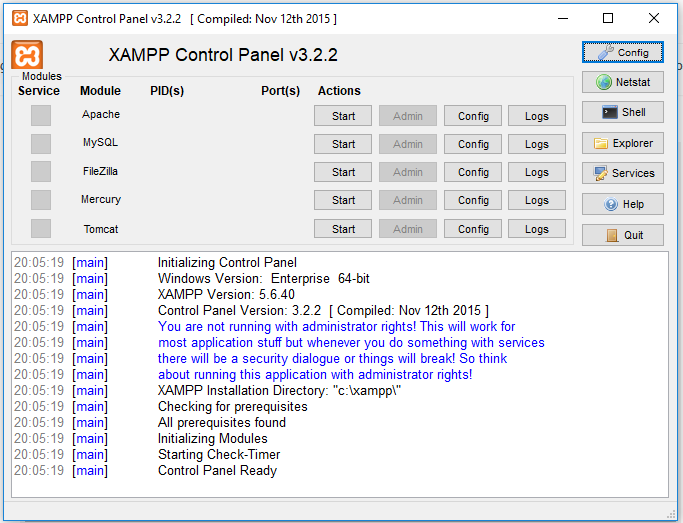
\includegraphics[width=0.5\textwidth]{figures/Xampp9.PNG}
    		\label{Xampp9}
		\end{figure}
\end{enumerate}

\section{Mengatasi Error Pada Xampp}

\chapter{CODEIGNITER}
Codeigniter adalah sebuah framework untuk web yang dibuat dalam format PHP. Format yang dibuat ini selanjutnya dapat digunakan untu membuat sistem aplikasi web yang kompleks. Codeigniter dapat mempercepat proses pembuatan web, karena semua class dan modul yang dibutuhkan sudah ada dan programmer hanya tinggal menggunakannya kembali pada aplikasi web yang akan dibuat \cite{prabowo2015website}.

\section{Tutorial Install CodeIgniter 3}
    \begin{enumerate}
        \item Pertama download Framework CodeIgniter di \textbf{\textit{https://www.codeigniter.com/}}
        
	    \item Setelah mengunduh file CodeIgniter 3, ekstrak file tersebut menggunakan WinRAR atau 7Zip kedalam folder \textit{C:/xampp/htdocs} jika kamu menggunakan XAMPP atau \textit{/var/www/html}. jika kamu menggunakan Apache2 Standalone, setelah itu ubahlan nama foldernya menjadi namaapplikasi.
	    
	    \item Sekarang silahkan Kamu coba akses URL \textbf{\textit{http://localhost/ namaaplikasi/}} melalui browser Kamu, akan langsung ditampilkan halaman awal Codeigniter yang berarti Instalasi telah berhasil.
		\begin{figure}[!htbp]
    		\centering
    		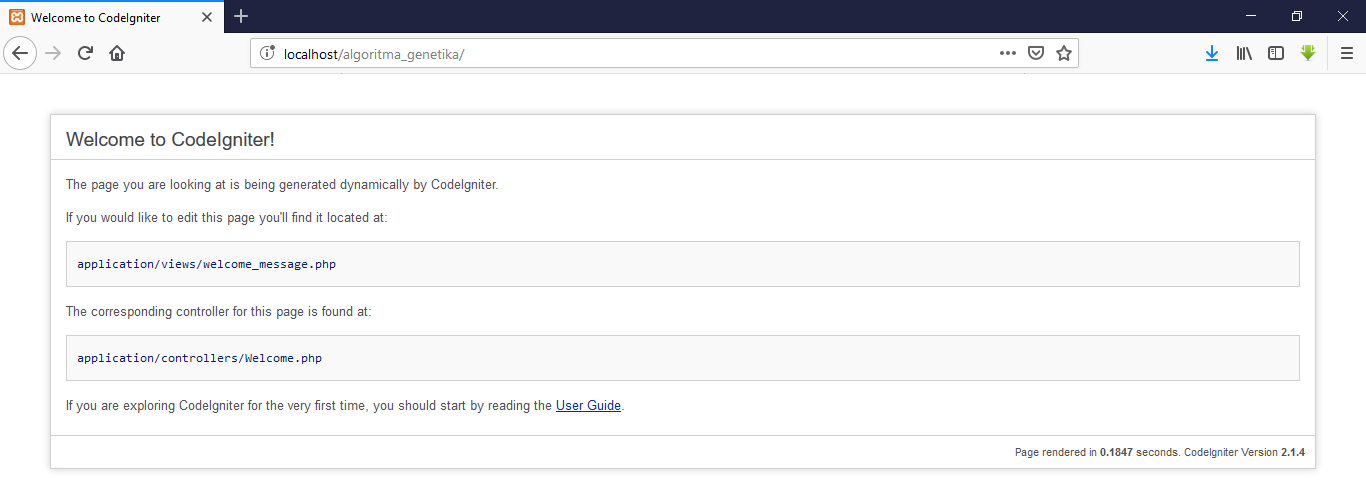
\includegraphics[width=0.5\textwidth]{figures/CodeIgniter1.PNG}
    		\label{CodeIgniter1}
		\end{figure}
    \end{enumerate}
    
\section{Struktur CodeIginter}
\begin{enumerate}
    \item Folder \textbf{Application}, merupakan folder yang pada dasarnya menyimpan aplikasi yang sedang kita buat
    \item Folder \textbf{Cache}, merupakan folder yang menyimpan semua cache yang dibuat oleh cache library
    \item Folder \textbf{Config}, merupakan folder yang menyimpan informasi mengenai konfigurasi aplikasi seperti autoload, database, routes dan lainnya.
    \item Folder \textbf{Controller}, merupakan folder menyimpan controller - controller aplikasi yang dapat digunakan untuk menyusun aktivitas program .
    \item Folder \textbf{Core}, adalah folder untuk memperluas class class inti codeigniter.
    \item Folder \textbf{Helpers}, merupakan folder untuk menyimpan helpers.
    \item Folder \textbf{Hooks}, merupakan folder untuk menyimpan hooks untuk mengubah alur fungsi dari core Codeigniter
    \item Folder \textbf{Language}, merupakan folder untuk menyimpan bahasa - bahasa yang akan digunakan.
    \item Folder \textbf{Libraries}, merupakan folder untuk menyimpan library.
    \item Folder \textbf{Logs}, merupakan folder untuk menyimpan semua error log apabila error log diaktifkan.
    \item Folder \textbf{Models}, merupakan folder untuk menyimpan models yang akan mendefinisikan tabel dari database yang dapat kita gunakan oleh Controller yang kita buat untuk mengakses database.
    \item Folder \verb|third_party|, merupakan folder untuk menyimpan fungsi fungsi tambahan dalam cara kerja codeigniter.
    \item Folder \textbf{Views}, merupakan folder untuk menyimpan tampilan dari aplikasi yang kita buat.
    \item Folder \textbf{System}, merupakan folder untuk menyimpan sistem inti dari Codeigniter.
\end{enumerate}

\section{Konfigurasi CodeIgniter 3}
Di dalam folder config pada CodeIgniter terdapat berbagai macam file konfigurasi yang dapat kita atur sendiri nantinya. File tersebut dapat ditemukan pada folder \textit{C:/xampp/htdocs/algoritmagenetika/application/config/}.
\begin{enumerate}
    \item \textbf{autoload.php}, digunakan untuk menambahkan package, libraries, drivers, helper, atau custom config lainnya agar secara otomatis diload oleh codeigniter.
    \item \textbf{config.php}, digunakan untuk membuat pengaturan dasar untuk web app codeigniter anda, seperti \verb|base_url|, index page, cookie, proxy dan lain lain.
    \item \textbf{constants.php}, digunakan untuk kita dapat membuat constant baru.
    \item \textbf{database.php}, digunakan untuk mengatur koneksi web app kita ke database.
    \item \textbf{doctypes.php}, sebagai tempat penyimpanan deklarasi dokumen Doctype.
    \item \verb|foreign_chars.php|, sebagai tempat penyimpanan karakter karakter asing.
    \item \textbf{hooks.php}, digunakan untuk mendefine "hooks" untuk meng extends CI
    \item \textbf{memcached.php}, config yang memungkinkan kita mencache database, driver dan lain lain sehingga lebih efektif.
    \item \textbf{migration.php}, config yang memungkinkan kita melakukan database migration. Secara default dijadikan False.
    \item \textbf{mimes.php}, menyimpan array yang berisi tipe file untuk fungsi upload.
    \item \textbf{profiler.php}, digunakan untuk mengatur profiler yang berguna pada saat debugging.
    \item \textbf{routes.php}, digunakan untuk mengatur default controllerdan overide 404
    \item \textbf{smileys.php}, menyimpan array yang berisi smiley yang membantu helper emoticon.
    \item \verb|user_agents.php|, menyimpan data user agent, yang membantu class User Agen untuk mengidentifikasi browser, platform, robotdan datamobile device
\end{enumerate}

Pada konfigurasi yang saya lakukan hanya melukakan konfigurasi pada file autoload.php, config.php, database.php dan routes.php. Berikut cara konfigurasinya:
\begin{enumerate}
    \item Autoload.php
		\par Pada file ini saya meng-input libraries untuk support framework CodeIgniter ini terhadap database, \verb|form_validation| yang akan dibuat nantinya, pagination dan Session untuk mengaktifkan session pada CodeIgniter. Pada variable autoload helper saya meng-input url dan form semua di inputkan sesuai dengan kebutuhan pembuat aplikasi. Array tersebut akan di eksekusi secara automatis oleh CodeIgniter.
\begin{lstlisting}
$autoload['libraries'] = array('database','session','form_validation','pagination');
$autoload['helper'] = array('url','form','html');
\end{lstlisting}

    \item Config.php
        \par Pada config.php inputkan url utama aplikasi pada variable config \verb|base_url| seperti pada codingan dibawah:
\begin{lstlisting}
$config['base_url']	= 'http://localhost/algoritma_genetika/';
\end{lstlisting}
        
    \item Database.php
		\par Pada database.php konfigurasi yang dilakukan untuk mengkoneksikan database yaitu MySQL dengan aplikasi web berbasis framework CodeIgniter. Dapat dilihat pada line 72, hostname yang diiniputkan sesuai dengan hostname yang dipakai, disini saya menginputkna localhost dengan username default yaitu root password dikosongkan karena pada Xampp saya tidak menggunakan password. Pada database line 75 inputkan nama database sesuai dengan nama database yang ada pada MySQL.
\begin{lstlisting}
$active_group = 'default';
$query_builder = TRUE;
$db['default'] = array(
	'dsn'	=> '',
	'hostname' => 'localhost',
	'username' => 'root',
	'password' => '',
	'database' => 'produk_ga_fs',
	'dbdriver' => 'mysqli',
	'dbprefix' => '',
	'pconnect' => FALSE,
	'db_debug' => (ENVIRONMENT !== 'production'),
	'cache_on' => FALSE,
	'cachedir' => '',
	'char_set' => 'utf8',
	'dbcollat' => 'utf8_general_ci',
	'swap_pre' => '',
	'encrypt' => FALSE,
	'compress' => FALSE,
	'stricton' => FALSE,
	'failover' => array(),
	'save_queries' => TRUE
);
\end{lstlisting}
		
	\item Routes.php
		\par Pada file ini dilakukan konfigurasi dimana controller mana yang akan pertama di eksekusi ketika url dijalankan.
\begin{lstlisting}
$route['default_controller'] = "CTRL_Dashboard";
$route['404_override'] = '';
\end{lstlisting}
\end{enumerate}

\section{Konfigurasi Bootstrap dan Template CodeIgniter 3}
Ada berbagai macam konfigurasi bootstrap dan template terhadap CodeIgniter, baik secara install maupun dengan cara konfigurasi sendiri. Pada tutorial kali ini saya ingin menerapkan bootstrap dan template di CodeIgniter dengan cara cepat. Untuk yang ingin menggunakan cara instan, bisa dengan cara mengunjungi website \textit{w3layout.com} dan website yang menyediakan assets template dan bootstrap siap pakai. Berikut cara konfigurasi template dan bootstrap pada CodeIgniter:
\begin{enumerate}
    \item Siapkan template bootstrap yang sudah didownload
    \item Extrak file tersebut jika dalam bentuk .rar atau .zip
    \item Buat folder baru dengan nama assets terhadap aplikasi yang ingin di konfigurasi kemudian copy file hasil extrak tadi ke dalam folder tersebut.
		\begin{figure}[!htbp]
    		\centering
    		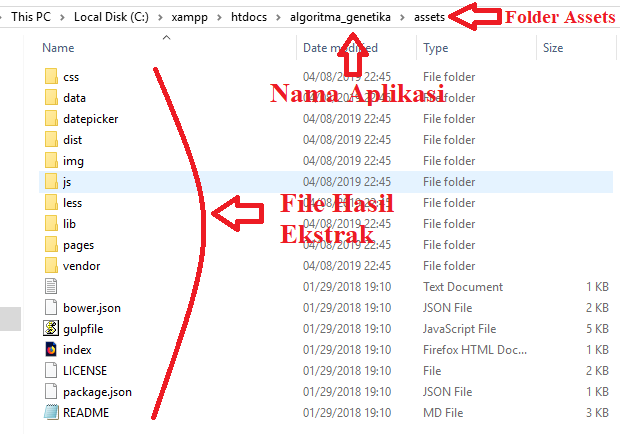
\includegraphics[width=0.5\textwidth]{figures/TBCI1.png}
    		\label{TBCI1}
		\end{figure}
		
	\item Setelah menkopi file kedalam folder assets, langka selanjutnya adalah memanggil config tersebut. Jangan lupa untuk membuat header dan footer ketika membuat website guna untuk mempermudah apabila terjadi perubahan terhadap beberapa menu.
	\item Copy isi dari index.html yang ada dalam assets kemudian buat file di dalam follder \textit{C:/xampp/htdocs/algoritmagenetika/application/views/dasboard.php} dengan format .php dan pastekan dalam file tersebut.
	\item Kemudian pisahkan antara header dan footer aplikasi anda.
	\item Pertama lakukan konfigurasi terhadap header dengan cara memanggil link dan script yang sudah di copy di dalam assets, berikut contoh pemanggilanya:
\begin{lstlisting}
<!DOCTYPE html>
<html lang="en">

<head>
    <meta charset="utf-8">
    <meta http-equiv="X-UA-Compatible" content="IE=edge">
    <meta name="viewport" content="width=device-width, initial-scale=1">
    <meta name="description" content="">
    <meta name="author" content="">

    <title>Penjadwalan Expediting</title>

    <link href="<?php echo base_url('assets/vendor/bootstrap/css/bootstrap.min.css'); ?>" rel="stylesheet">
    <link href="<?php echo base_url('assets/vendor/metisMenu/metisMenu.min.css'); ?>" rel="stylesheet">
    <link href="<?php echo base_url('assets/dist/css/sb-admin-2.css'); ?>" rel="stylesheet">
    <link href="<?php echo base_url('assets/vendor/morrisjs/morris.css'); ?>" rel="stylesheet">
    <link href="<?php echo base_url('assets/vendor/font-awesome/css/font-awesome.min.css'); ?>" rel="stylesheet" type="text/css">
    <script src="<?php echo base_url('assets/vendor/jquery/jquery.min.js'); ?>"></script>

    <!-- Tabel Responsive -->
    <link href="<?php echo base_url('assets/vendor/datatables-plugins/dataTables.bootstrap.css'); ?>" rel="stylesheet">
    <link href="<?php echo base_url('assets/vendor/datatables-responsive/dataTables.responsive.css'); ?>" rel="stylesheet">

    <!-- DatePicker -->
    <link href="<?php echo base_url('assets/datepicker/datepicker.css'); ?>" rel="stylesheet">
    <script type="text/javascript" src="<?php echo base_url('assets/datepicker/datepicker.js'); ?>"></script>

    <style type="text/css">
         body .frmModalMsg {
            width: 740px;
            margin-left: -280px;
         }
   
         #line-chart {
            height:300px;
            width:800px;
            margin: 0px auto;
            margin-top: 1em;
         }
         .brand { font-family: georgia, serif; }
         .brand .first {
         color: #ccc;
            font-style: italic;
         }
         .brand .second {
            color: #fff;
            font-weight: bold;
         }
         
         #loading-div-background{
            display: none;
            position: fixed;
            top: 0;
            left: 0;
            background: #fff;
            width: 100%;
            height: 100%;
        }
        
        #loading-div{
            width: 300px;
            height: 150px;
            background-color: #fff;
            border: 5px solid #1468b3;
            text-align: center;
            color: #202020;
            position: absolute;
            left: 50%;
            top: 50%;
            margin-left: -150px;
            margin-top: -100px;
            -webkit-border-radius: 5px;
            -moz-border-radius: 5px;
            border-radius: 5px;
        }
      </style>

      <script type="text/javascript">
        $(document).ready(function (){
            $("#loading-div-background").css({ opacity: 0.5 });
         <?php if(isset($clear_text_box)) { ?>    
            $('input[type=text]').each(function() {
                $(this).val('');
            });
         <?php } ?>
        });
    
        function ShowProgressAnimation(){
            $("#loading-div-background").show();
        }
         
         function change_get(){     
            var semester_tipe = document.getElementById('semester_tipe');
            var tahun_akademik = document.getElementById('tahun_akademik');
            window.location.href = "<?php echo base_url().'web/pengampu/' ?>" + semester_tipe.options[semester_tipe.selectedIndex].value  + "/"   + tahun_akademik.options[tahun_akademik.selectedIndex].value;     
         }
         
         function change_dosen_tidak_bersedia() {
            var kode_dosen = document.getElementById('kode_dosen');         
            window.location.href = "<?php echo base_url().'web/waktu_tidak_bersedia/' ?>" + kode_dosen.options[kode_dosen.selectedIndex].value;     
         }
         
        function get_matakuliah() {        
            var semester_tipe = document.getElementById('semester_tipe');
            $.ajax({
               type:"POST",
               async   : false,
               cache   : false,
               url: "<?php echo base_url()?>web/option_matakuliah_ajax/" + semester_tipe.options[semester_tipe.selectedIndex].value,
               success: function(msg){
                  //alert(msg);
                  $('#option_matakuliah').html(msg);
               }
            });
            return false;        
        }

        function delete_row(link,kode) {
            var answer =  confirm('Anda yakin ingin menghapus data ini?');
            if(answer){
               $.ajax({
                  type:"POST",
                  async   : false,
                  cache   : false,
                  url: "<?php echo base_url()?>" + link + kode,
                  success: function(msg){
                     var tr  = $('#row_' + kode);
                     tr.css("background-color","#FF3700");
                     tr.fadeOut(400, function(){
                       tr.remove();
                     });                  
                  }
               });
            }
            return false;
        }
        
        $(function() {
                applyPagination();
                function applyPagination() {
                 $("#ajax_paging a").click(function() {             
                   var url = $(this).attr("href");
                   $.ajax({
                     type: "POST",
                     data: "ajax=1",
                     url: url, 
                     success: function(msg) {
                       $('#content_ajax').fadeOut(0,function(){
                           $('#content_ajax').html(msg);
                           $("#content_ajax").removeAttr("style");
                           applyPagination();                 
                       }).fadeIn(0);                       
                     }
                   });              
                   return false;
                 });
               }
             });
      </script>
</head>

<body>
    <div id="wrapper">
        <nav class="navbar navbar-default navbar-static-top" role="navigation" style="margin-bottom: 0">
            <div class="navbar-header">
                <button type="button" class="navbar-toggle" data-toggle="collapse" data-target=".navbar-collapse">
                    <span class="sr-only">Toggle navigation</span>
                    <span class="icon-bar"></span>
                    <span class="icon-bar"></span>
                    <span class="icon-bar"></span>
                </button>
                <a class="navbar-brand" href="<?php echo base_url();?>">Algoritma Genetika</a>
            </div>

            <div class="navbar-default sidebar" role="navigation">
                <div class="sidebar-nav navbar-collapse">
                    <ul class="nav" id="side-menu">
                        <li>
                            <a href="<?php echo base_url();?>"><i class="fa fa-dashboard fa-fw"></i> Dashboard</a>
                        </li>
                        <li>
                            <a href="#"><i class="fa fa-files-o fa-fw"></i> Data<span class="fa arrow"></span></a>
                            <ul class="nav nav-second-level">
                                <li>
                                    <?php echo anchor('Web/index_vendor', '<i class="fa fa-file-text fa-fw"></i> Vendor'); ?>
                                </li>
                                <li>
                                    <?php echo anchor('Web/index_barang', '<i class="fa fa-file-text fa-fw"></i> Barang'); ?>
                                </li>
                                <li>
                                    <?php echo anchor('Web/index_bulan_tahun', '<i class="fa fa-file-text fa-fw"></i> Bulan Dan Tahun'); ?>
                                </li>
                            </ul>
                        </li>
                        <li>
                            <?php echo anchor('web/index_jadwal', '<i class="fa fa-table fa-fw"></i> Jadwal'); ?>
                        </li>
                    </ul>
                </div>
            </div>
        </nav>
\end{lstlisting}
		\par Lakukan pemanggilan terhadap semua code yang berbau href dan src dengan mengisikan kodingan seperti echo \verb|base_url/assets/link_yg_dituju|, terlihat seperti pada codingan diatas. Lakukan hal yang sama terhadap file footer.php. Setelah itu simpan.
		
	\item Selanjutnya membuat file untuk tampilan awal yaitu dashboard.php
	\item Edit codingan yang sudah dipastekan pada file dashboard.php yang ada pada folder \textit{C:/xampp/htdocs/algoritmagenetika/application/views/} sesuai tampilan yang diinginkan. Apabila memisahkan file header dan footer jangan lupa untuk memanggil file tersebut. Berikut codingan full dari dasboard.php:
\begin{lstlisting}
<?php $this->load->view('page/header') ?>

<div id="page-wrapper">
    <div class="row">
        <div class="col-lg-12">
            <h1 class="page-header">Dashboard</h1>
        </div>
    </div>
    <div class="row">
        <div class="col-lg-3 col-md-6">
            <div class="panel panel-primary">
                <div class="panel-heading">
                    <div class="row">
                        <div class="col-xs-3">
                            <i class="fa fa-tasks fa-5x"></i>
                        </div>
                        <div class="col-xs-9 text-right">
                            <div class="huge">Data</div>
                            <div>Vendor</div>
                        </div>
                    </div>
                </div>
                <a href="<?php echo base_url()?>index.php/Web/index_vendor">
                    <div class="panel-footer">
                        <span class="pull-left">View Details</span>
                        <span class="pull-right"><i class="fa fa-arrow-circle-right"></i></span>
                        <div class="clearfix"></div>
                    </div>
                </a>
            </div>
        </div>
        <div class="col-lg-3 col-md-6">
            <div class="panel panel-green">
                <div class="panel-heading">
                    <div class="row">
                        <div class="col-xs-3">
                            <i class="fa fa-tasks fa-5x"></i>
                        </div>
                        <div class="col-xs-9 text-right">
                            <div class="huge">Data</div>
                            <div>Barang</div>
                        </div>
                    </div>
                </div>
                <a href="<?php echo base_url()?>index.php/Web/index_barang">
                    <div class="panel-footer">
                        <span class="pull-left">View Details</span>
                        <span class="pull-right"><i class="fa fa-arrow-circle-right"></i></span>
                        <div class="clearfix"></div>
                    </div>
                </a>
            </div>
        </div>
        <div class="col-lg-3 col-md-6">
            <div class="panel panel-yellow">
                <div class="panel-heading">
                    <div class="row">
                        <div class="col-xs-3">
                            <i class="fa fa-tasks fa-5x"></i>
                        </div>
                        <div class="col-xs-9 text-right">
                            <div class="huge">Data</div>
                            <div>Bulan Dan Tahun</div>
                        </div>
                    </div>
                </div>
                <a href="<?php echo base_url()?>index.php/Web/index_bulan_tahun">
                    <div class="panel-footer">
                        <span class="pull-left">View Details</span>
                        <span class="pull-right"><i class="fa fa-arrow-circle-right"></i></span>
                        <div class="clearfix"></div>
                    </div>
                </a>
            </div>
        </div>
        <div class="col-lg-3 col-md-6">
            <div class="panel panel-red">
                <div class="panel-heading">
                    <div class="row">
                        <div class="col-xs-3">
                            <i class="fa fa-table fa-5x"></i>
                        </div>
                        <div class="col-xs-9 text-right">
                            <div class="huge">Data</div>
                            <div>Jadwal</div>
                        </div>
                    </div>
                </div>
                <a href="<?php echo base_url()?>index.php/Web/index_jadwal">
                    <div class="panel-footer">
                        <span class="pull-left">View Details</span>
                        <span class="pull-right"><i class="fa fa-arrow-circle-right"></i></span>
                        <div class="clearfix"></div>
                    </div>
                </a>
            </div>
        </div>
    </div>

    <div class="row">
    </div>
</div>

<?php $this->load->view('page/footer') ?>
\end{lstlisting}
	    \par Load view berarti meload file yang ada di dalam folder view, dalam artian codingan diatas akan meload file header yang ada di folder \textit{application/views/page/header.php}, begitu juga dengan file \textit{footer.php}. Simpan semua konfigurasi kemudian  jalankan aplikasi algoritmagenetika tersebut, dengan cara ketik link \textit{http://localhost/algoritmagenetika/} di browser kesayangan anda.
	    
    \item Berikut hasil dari codingan dashboard.php.
		\begin{figure}[!htbp]
    		\centering
    		\caption{Tampilan Awal Template / Bootsrap CodeIgniter 3}
    		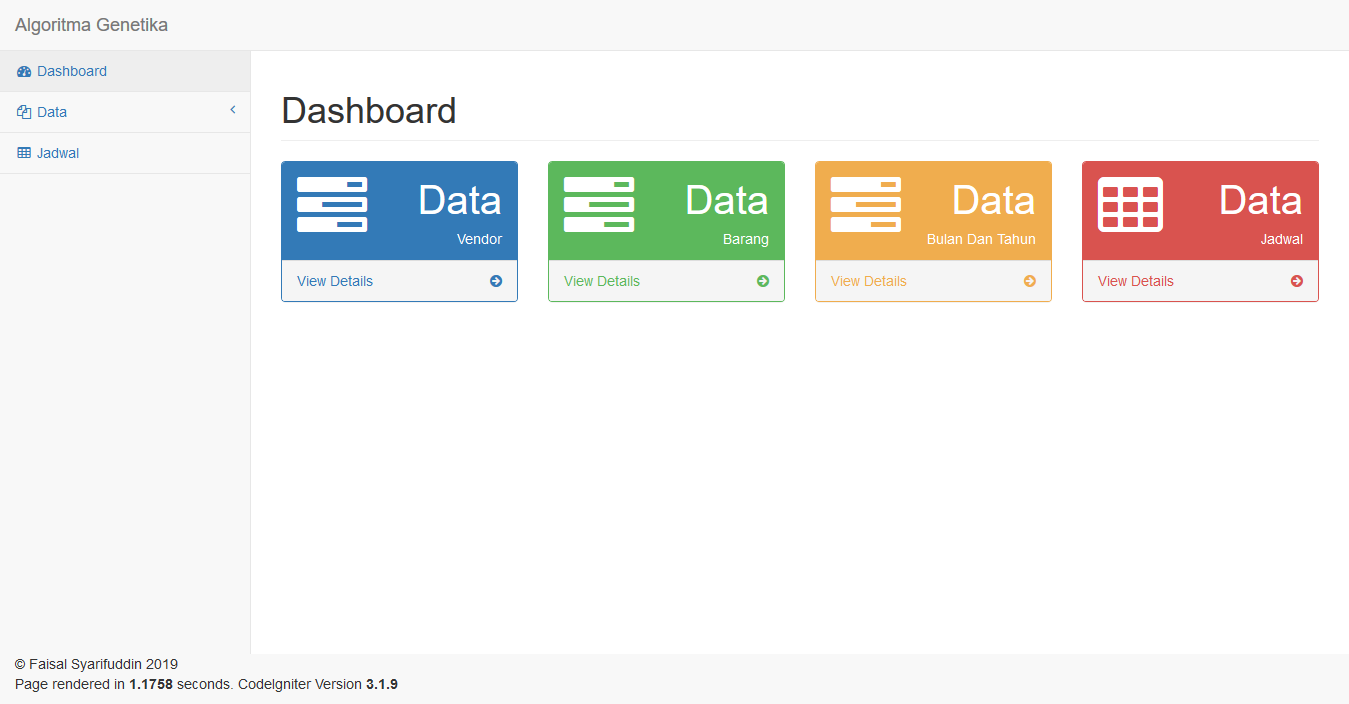
\includegraphics[width=0.5\textwidth]{figures/TBCI3.png}
    		\label{TBCI3}
		\end{figure}
\end{enumerate}

\section{MVC dan CRUD CodeIgniter 3}
\begin{enumerate}
    \item Konfigurasi Model
    \begin{enumerate}
        \item Buat table sesuai dengan kebutuhan aplikasi
        \item Kemudian buat file baru dengan nama \verb|MDL_Barang.php| dalam folder \textit{C:/xampp/htdocs/algoritmagenetika/application/models/}.
        \item Pada tahap ini saya akan membuat model untuk table barang, berikut codingan yang saya gunakan:
\begin{lstlisting}
<?php
class MDL_Barang extends CI_Model{
	function __construct(){
		parent::__construct();
	}
    
    public function get_barang(){
		$hasil=$this->db->get('barang');
		if($hasil->num_rows() > 0){
			return $hasil->result();
		}else{
			return false;
        }
    }

	public function insert_barang($barang_data)
	{
		$this->db->insert('barang',$barang_data);
	}

	public function find_barang($kode_barang)
	{
		$hasil = $this->db->where('kode_barang',$kode_barang)->limit(1)->get('barang');
		if($hasil->num_rows() > 0){
			return $hasil->row();
		}else{
			return array();
		}
	}

	public function update_barang($kode_barang, $barang_data)
	{
		$this->db->where('kode_barang',$kode_barang)
		->update('barang',$barang_data);	
	}
	
	public function delete_barang($kode_barang)
	{
		$this->db->where('kode_barang',$kode_barang)
		->delete('barang');
	}

	public function detail_barang($kode_barang)
	{
		$hasil = $this->db->where('kode_barang',$kode_barang)->limit(1)->get('barang');
		if($hasil->num_rows() > 0){
			return $hasil->result();
		}else{
			return array();
		}
	}
}
\end{lstlisting}
            
        \par Penjelasan:
        \begin{enumerate}
            \item function \verb|get_barang| berfungsi untuk meload semua data yang ada di database barang
            \item function \verb|insert_barang| berfungsi untuk melakukan execute insert data ke dalam table barang
            \item function \verb|find_barang| berfungsi untuk mencari kode barang yang akan di edit
            \item function \verb|update_barang| berfungsi untuk melakukan execute update terhadap table barang
            \item function \verb|delete_barang| berfungsi untuk melakukan execute delete data pada table barang
            \item function \verb|detail_barang| berfungsi untuk melihat data lengkap barang sesuai dengan id yang dipanggil.
            
            \par Function-function di atas merupakan function dasar untuk melakukan proses CRUD di model CodeIgniter 3.
        \end{enumerate}
    \end{enumerate}
    
    \item Konfigurasi Controller
    \begin{enumerate}
        \item Buat file baru dengan nama web pada folder \textit{C/xampp/htdocs/algoritmagenetika/application/controllers/}, kemudian buat beberapa function crud.
        \item Dalam file web.php, load semua model agar semua function disatukan dalam satu file, seperti pada codingan dibawah:
\begin{lstlisting}
<?php if (!defined('BASEPATH')) exit('No direct script access allowed');
class Web extends CI_Controller
{
	function __construct()
    {
        parent::__construct();
		$this->load->model(array('MDL_Vendor',
								 'MDL_Barang',
								 'MDL_Bulan_Tahun',
								 'MDL_Hari',
								 'MDL_Jam',
								 'MDL_Pengampu',
								 'MDL_Waktu_Tidak_Bersedia',
								 'MDL_Jadwal'));
		include_once("genetik.php");
		define('IS_TEST','FALSE');
    }
\end{lstlisting}
    		
    	\item Kemudian buat function pertama yaitu function \verb|index_barang|, untuk menampilakn seluruh data yang ada pada table barang.
\begin{lstlisting}
public function index_barang(){
    $data['barang'] = $this->MDL_Barang->get_barang();
    $this->load->view('web/barang/index_barang', $data);
}
\end{lstlisting}
    		
        \item Function kedua yaitu function \verb|add_barang|, untuk melakukan proses input data dalam bentuk variable sesuai dengan field yang ada pada table barang  yang kemudian variable tersebut akan di lempar ke model untuk di inputkan kedalam table.
\begin{lstlisting}
public function add_barang()
{
	$this->form_validation->set_rules('nama_barang','Nama barang','required');
	$this->form_validation->set_rules('kategori_barang','Kategori Barang','required');
	$this->form_validation->set_rules('tingkat_kebutuhan','Tingkat Kebutuhan','required');
	$this->form_validation->set_rules('jumlah_dalam_kategori','Jumlah Dalam Kategori','required');
	
	if($this->form_validation->run() == FALSE){
        $this->load->view('web/barang/form_add_barang');
	}else{
		$barang_data = array (
			'nama_barang'			=> set_value('nama_barang'),
			'kategori_barang'		=> set_value('kategori_barang'),
			'tingkat_kebutuhan'		=> set_value('tingkat_kebutuhan'),
			'jumlah_dalam_kategori'	=> set_value('jumlah_dalam_kategori')
		);
		$this->MDL_Barang->insert_barang($barang_data);
		$this->session->set_flashdata('notif','Data Berhasil Di Simpan');
		redirect('web/index_barang');	
	}
}
\end{lstlisting}
    		
    	\item Selanjutnya function \verb|edit_barang|, untuk melakukan proses edit data barang yang kemudian variable yang di tampung akan di execute pada model function \verb|update_barang|.
\begin{lstlisting}
public function edit_barang($kode_barang)
{
	$this->form_validation->set_rules('nama_barang','Nama barang','required');
	$this->form_validation->set_rules('kategori_barang','Kategori Barang','required');
	$this->form_validation->set_rules('tingkat_kebutuhan','Tingkat Kebutuhan','required');
	$this->form_validation->set_rules('jumlah_dalam_kategori','Jumlah Dalam Kategori','required');
	
	if($this->form_validation->run() == FALSE){
		$data['barang'] = $this->MDL_Barang->find_barang($kode_barang);
		$this->load->view('web/barang/form_edit_barang', $data);
	}else{
		$barang_data = array (
			'nama_barang'			=> set_value('nama_barang'),
			'kategori_barang'		=> set_value('kategori_barang'),
			'tingkat_kebutuhan'		=> set_value('tingkat_kebutuhan'),
			'jumlah_dalam_kategori'	=> set_value('jumlah_dalam_kategori')
		);
		$this->MDL_Barang->update_barang($kode_barang, $barang_data);
		redirect('web/index_barang');
	}	
}
\end{lstlisting}
    		
    	\item Function \verb|delete_barang|, untuk melakukan hapus data berdasarkan id yang di execute.
\begin{lstlisting}
public function delete_barang($kode_barang)
{
	$this->MDL_Barang->delete_barang($kode_barang);
	redirect('web/index_barang');	
}
\end{lstlisting}
    \end{enumerate}
    
    \item Konfigurasi Views
    \begin{enumerate}
        \item Buat file dengan nama \verb|index_barang.php| pada folder \textit{C/xampp/htdocs/algoritmagenetika/application/views/web/barang/} kemdian buat desain untuk menampilkan data dari table barang, berikut contoh codingan untuk vies data barang.
\begin{lstlisting}
<?php $this->load->view('page/header') ?>
    <div id="page-wrapper">
        <div class="row">
            <div class="col-lg-12">
                <h1 class="page-header">Barang</h1>
            </div>
        </div>

        <div class="row">
            <div class="col-lg-12">
                <ol class="breadcrumb">
                    <?=anchor('Web/add_barang','Tambah Data Barang',['class'=>'btn btn-primary btn-sm','style'=>'float:left;'])?>
                    <div style="clear: both;"></div>
                </ol>
            </div>
        </div>

        <div class="row">
            <div class="container table-responsive">
                <div class="col-lg-11">
                    <table id="dataTables-example" class="table table-hover">
                    <thead>
                        <tr>
                            <th class="header">Nama Barang</th>
                            <th class="header">Kategori Barang</th>
                            <th class="header">#</th>
                        </tr>
                    </thead>
                    <tbody>
                        <?php foreach($barang as $row) : ?> 
                        <tr>
                            <td><?=$row->nama_barang?></td>
                            <td><?=$row->kategori_barang?></td>
                            <td>
                                <center>
                                    <?=anchor('Web/detail_barang/' . $row->kode_barang,'Detail',['class'=>'btn btn-info btn-sm'])?>
                                    <?=anchor('Web/edit_barang/' . $row->kode_barang,'Ubah',['class'=>'btn btn-default btn-sm'])?>
                                    <?=anchor('Web/delete_barang/' . $row->kode_barang,'Hapus',['class'=>'btn btn-danger btn-sm','onclick'=>'return confirm(\'Apakah Anda Yakin ?\')'])?>
                                </center>
                            </td>
                        </tr>
                        <?php endforeach; ?>
                    </tbody>
                    </table>
                </div>
            </div>
        </div>
    </div>
<?php $this->load->view('page/footer') ?>
\end{lstlisting}
    		
    	\item Selanjutnya membuat file baru didalam folder yang sama, dengan nama file \verb|form_add_barang.php|, untuk view terhadap function tambah barang.
\begin{lstlisting}
<?php $this->load->view('page/header') ?>
    <div id="page-wrapper">
        <div class="row">
            <div class="col-lg-12">
                <h1 class="page-header">Tambah Data Barang</h1>
                <ol class="breadcrumb">
                  <li><?php echo anchor('web/index_barang', '<i class="fa fa-file-text fa-fw"></i> Data Barang'); ?></li>
                  <li class="active"><i class="fa fa-tasks fa-fw"></i> Tambah Data Barang</li>
                  
                  <div style="clear: both;"></div>
                </ol>
            </div>
        </div>

        <div class="row">
            <div class="col-lg-11">
                <?=form_open_multipart('web/add_barang/',['class'=>'form-horizontal'])?>

                    <?php $error = form_error("nama_barang", "<p class='text-danger'>", '</p>'); ?>
                    <div class="form-group <?php echo $error ? 'has-error' : '' ?>">
                        <label class="col-sm-2 control-label">Nama barang</label>
                        <div class="col-sm-10">
                            <input type="text" class="form-control" name="nama_barang" value="<?= set_value('nama_barang') ?>">
                        </div>
                    </div>
                    <?php echo $error; ?>

                    <?php $error = form_error("kategori_barang", "<p class='text-danger'>", '</p>'); ?>
                    <div class="form-group <?php echo $error ? 'has-error' : '' ?>">
                        <label class="col-sm-2 control-label">Kategori Barang</label>
                        <div class="col-sm-10">
                            <select class="form-control" name="kategori_barang">
                                <option value=''>--Pilih Kategori Barang--</option>
                                <option value='Piping'>Piping</option>
                                <option value='Mechanical'>Mechanical</option>
                                <option value='Instrument'>Instrument</option>
                                <option value='Electrical'>Electrical</option>
                                <option value='Safety'>Safety</option>
                            </select>
                        </div>
                    </div>
                    <?php echo $error; ?>

                    <?php $error = form_error("tingkat_kebutuhan", "<p class='text-danger'>", '</p>'); ?>
                    <div class="form-group <?php echo $error ? 'has-error' : '' ?>">
                        <label class="col-sm-2 control-label">Tingkat Kebutuhan</label>
                        <div class="col-sm-10">
                            <select class="form-control" name="tingkat_kebutuhan">
                                <option value=''>--Pilih Tingkat Kebutuhan--</option>
                                <option value='1'>1 (Dibutuhkan Paling Akhir)</option>
                                <option value='2'>2 (Dibutuhkan Setelah Point 3 Selesai)</option>
                                <option value='3'>3 (Dibutuhkan Setelah Barang Utama Datang)</option>
                                <option value='4'>4 (Dibutuhkan Paling Utama)</option>
                            </select>
                        </div>
                    </div>
                    <?php echo $error; ?>

                    <?php $error = form_error("jumlah_dalam_kategori", "<p class='text-danger'>", '</p>'); ?>
                    <div class="form-group <?php echo $error ? 'has-error' : '' ?>">
                        <label class="col-sm-2 control-label">Jumlah Dalam Kategori</label>
                        <div class="col-sm-10">
                            <select class="form-control" name="jumlah_dalam_kategori">
                                <option value=''>--Pilih Jumlah Dalam Kategori--</option>
                                <option value='1'>Kurang Dari 10 Barang</option>
                                <option value='2'>Kurang Dari 20 Barang</option>
                                <option value='3'>Kurang Dari 30 Barang</option>
                                <option value='4'>Kurang Dari 40 Barang</option>
                                <option value='5'>Kurang Dari 50 Barang</option>
                                <option value='6'>Kurang Dari 60 Barang</option>
                                <option value='7'>Kurang Dari 70 Barang</option>
                                <option value='8'>Kurang Dari 80 Barang</option>
                            </select>
                        </div>
                    </div>
                    <?php echo $error; ?>

                    <div class="form-group">
                        <div class="col-sm-offset-2 col-sm-10">
                            <button type="submit" class="btn btn-primary pull-right">Simpan</button>
                        </div>
                    </div>
               </form>
            </div>
        </div>
        
    </div>
<?php $this->load->view('page/footer') ?>

\end{lstlisting}
    		\par Jangan lupa untuk menutup form dan pastikan name pada codingan views sesuai dengan data variable yang akan di execute pada function \verb|add_barang| yang terdapat pada controller tadi.
    		
    	\item Masih dalam folder yang saya, buat file baru untuk views terhadap function edit data barang dengan nama \verb|form_edit_barang.php|. Pada edit barang, hal pertama yang harus dilakukan setelah menekan tombol edit barang adalah memanggil semua data yang ada pada table agar dapat diedit, berikut contoh pemanggilan data pada form edit data barang.
\begin{lstlisting}
<?php
$kode_barang    = $barang->kode_barang;
    if($this->input->post('is_submitted')){
        $nama_barang            = set_value('nama_barang');
        $kategori_barang        = set_value('kategori_barang');
        $tingkat_kebutuhan      = set_value('tingkat_kebutuhan');
        $jumlah_dalam_kategori  = set_value('jumlah_dalam_kategori');
    }else{
        $nama_barang            = $barang->nama_barang;
        $kategori_barang        = $barang->kategori_barang;
        $tingkat_kebutuhan      = $barang->tingkat_kebutuhan;
        $jumlah_dalam_kategori  = $barang->jumlah_dalam_kategori;
    }
?>
\end{lstlisting}
    		
    		\par Setelah memanggil variable yang akan diedit, dibawah codingan tersebut buat form untuk view function edit data barang.
\begin{lstlisting}
<?php $this->load->view('page/header') ?>
    <div id="page-wrapper">
        <div class="row">
            <div class="col-lg-12">
                <h1 class="page-header">Tambah Data barang</h1>
                <ol class="breadcrumb">
                  <li><?php echo anchor('web/index_barang', '<i class="fa fa-file-text fa-fw"></i> Data Barang'); ?></li>
                  <li class="active"><i class="fa fa-tasks fa-fw"></i> Edit Data Barang</li>
                  <div style="clear: both;"></div>
                </ol>
            </div>
        </div>

        <div class="row">
            <div class="col-lg-11">
                <?=form_open_multipart('web/edit_barang/' . $kode_barang,['class'=>'form-horizontal'])?>

                    <?php $error = form_error("nama_barang", "<p class='text-danger'>", '</p>'); ?>
                    <div class="form-group <?php echo $error ? 'has-error' : '' ?>">
                        <label class="col-sm-2 control-label">Nama barang</label>
                        <div class="col-sm-10">
                            <input type="text" class="form-control" name="nama_barang" value="<?= $nama_barang ?>">
                        </div>
                    </div>
                    <?php echo $error; ?>

                    <?php $error = form_error("kategori_barang", "<p class='text-danger'>", '</p>'); ?>
                    <div class="form-group <?php echo $error ? 'has-error' : '' ?>">
                        <label class="col-sm-2 control-label">Kategori barang</label>
                        <div class="col-sm-10">
                            <select class="form-control" name="kategori_barang">
                                <option value='<?= $kategori_barang ?>'><?= $kategori_barang ?></option>
                                <option value='Piping'>Piping</option>
                                <option value='Mechanical'>Mechanical</option>
                                <option value='Instrument'>Instrument</option>
                                <option value='Electrical'>Electrical</option>
                                <option value='Safety'>Safety</option>
                            </select>
                        </div>
                    </div>
                    <?php echo $error; ?>

                    <?php $error = form_error("tingkat_kebutuhan", "<p class='text-danger'>", '</p>'); ?>
                    <div class="form-group <?php echo $error ? 'has-error' : '' ?>">
                        <label class="col-sm-2 control-label">Tingkat Kebutuhan</label>
                        <div class="col-sm-10">
                            <select class="form-control" name="tingkat_kebutuhan">
                                <option value='<?= $tingkat_kebutuhan ?>'><?= $tingkat_kebutuhan ?></option>
                                <option value='1'>1 (Dibutuhkan Paling Akhir)</option>
                                <option value='2'>2 (Dibutuhkan Setelah Point 3 Selesai)</option>
                                <option value='3'>3 (Dibutuhkan Setelah Barang Utama Datang)</option>
                                <option value='4'>4 (Dibutuhkan Paling Utama)</option>
                            </select>
                        </div>
                    </div>
                    <?php echo $error; ?>

                    <?php $error = form_error("jumlah_dalam_kategori", "<p class='text-danger'>", '</p>'); ?>
                    <div class="form-group <?php echo $error ? 'has-error' : '' ?>">
                        <label class="col-sm-2 control-label">Jumlah Dalam Kategori</label>
                        <div class="col-sm-10">
                            <select class="form-control" name="jumlah_dalam_kategori">
                                <option value='<?= $jumlah_dalam_kategori ?>'><?= $jumlah_dalam_kategori ?></option>
                                <option value='1'>Kurang Dari 10 Barang</option>
                                <option value='2'>Kurang Dari 20 Barang</option>
                                <option value='3'>Kurang Dari 30 Barang</option>
                                <option value='4'>Kurang Dari 40 Barang</option>
                                <option value='5'>Kurang Dari 50 Barang</option>
                                <option value='6'>Kurang Dari 60 Barang</option>
                                <option value='7'>Kurang Dari 70 Barang</option>
                                <option value='8'>Kurang Dari 80 Barang</option>
                            </select>
                        </div>
                    </div>
                    <?php echo $error; ?>

                    <div class="form-group">
                        <div class="col-sm-offset-2 col-sm-10">
                            <button type="submit" class="btn btn-primary pull-right">Simpan</button>
                        </div>
                    </div>
               </form>
            </div>
        </div>
        
    </div>
<?php $this->load->view('page/footer') ?>
\end{lstlisting}
    		\par Pastikan value terisi, agar saat melakukan edit data, yang diedit dapat terlihat dan pastikan pada name sesuai dengan field yang ada pada table dan function \verb|edit_barang| yang ada pada folder controller.
    		
    	\item Simpan semua file tersebut kemudian jalankan aplikasi ini dengan load link \textit{http://localhost/algoritmagenetika/} pada browser kesayangan anda (jangan lupa untuk jalankan apache dan mysql xampp terlebih dahulu). Berikut tampilan CRUD dari codingan yang di buat.
    	\begin{enumerate}
    	    \item Views Barang
    		\begin{figure}[!htbp]
        		\centering
        		\caption{Tampilan Hasil MVC dan CRUD (Views Barang)}
        		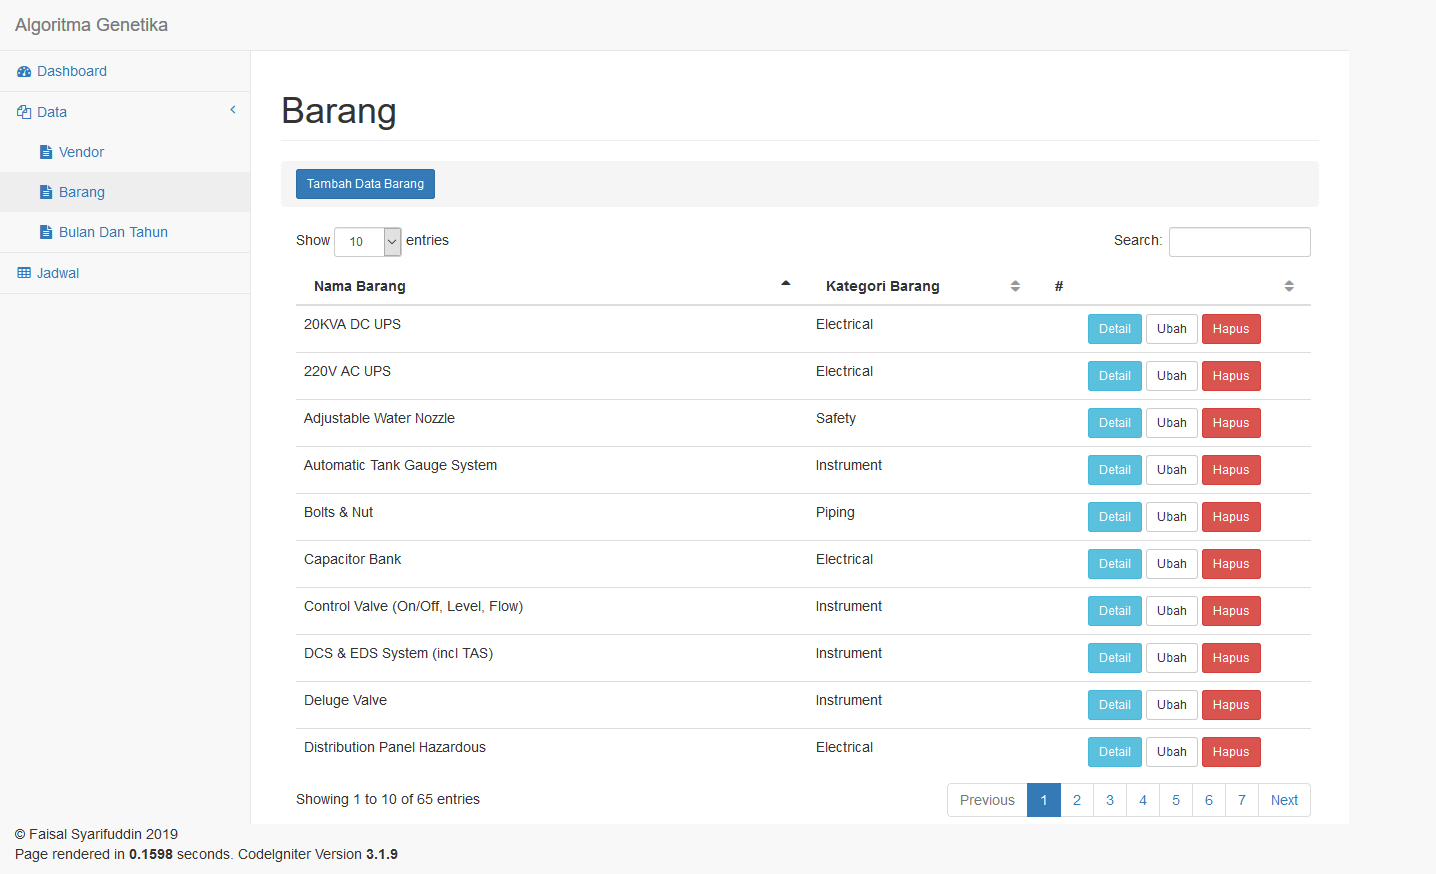
\includegraphics[width=0.4\textwidth]{figures/Views5.png}
        		\label{Views5}
    		\end{figure}
    		
    		\item Views Tambah Barang
    		\begin{figure}[!htbp]
        		\centering
        		\caption{Tampilan Hasil MVC dan CRUD (Tambah Barang)}
        		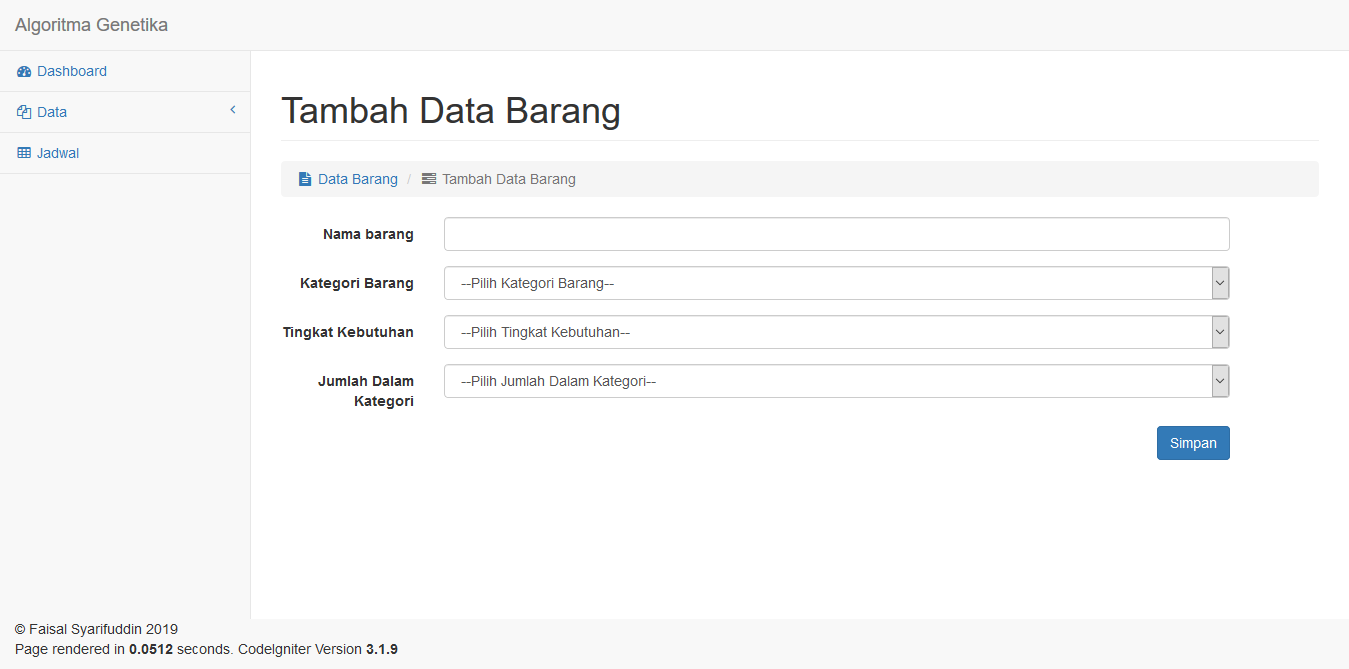
\includegraphics[width=0.4\textwidth]{figures/Views6.png}
        		\label{Views6}
    		\end{figure}
    		
    		\item Views Edit Barang
    		\begin{figure}[!htbp]
        		\centering
        		\caption{Tampilan Hasil MVC dan CRUD (Edit Barang)}
        		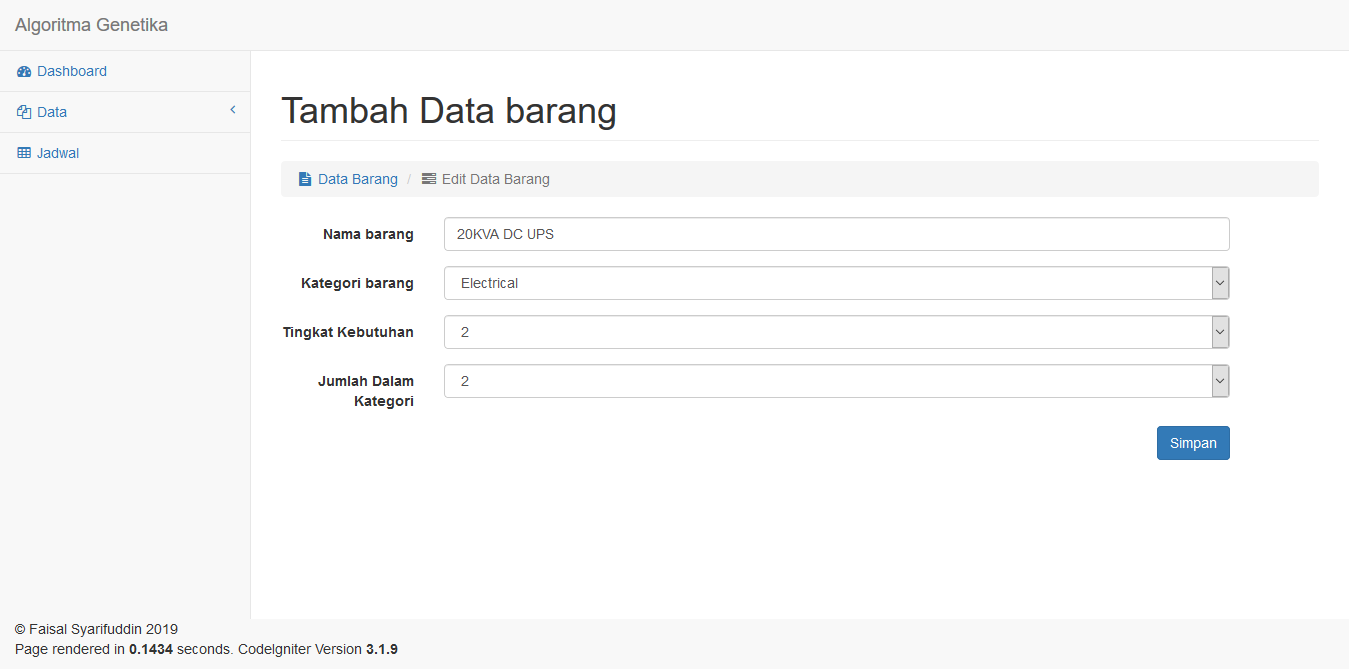
\includegraphics[width=0.4\textwidth]{figures/Views7.png}
        		\label{Views7}
    		\end{figure}
    	\end{enumerate}
    \end{enumerate}
\end{enumerate}

\chapter{ALGORITMA GENETIKA}
Algoritma Genetika (GA) merupakan salah satu metode heuristic yang merupakan cabang dari evolutionary algorithm, yaitu suatu teknik untuk memecahkan masalah-masalah optimasi yang rumit dengan menirukan proses evolusi mahluk hidup. GA terbukti sesuai digunakan untuk menyelesaikan masalah multi objektif. GA berkembang seiring dengan perkembangan teknologi informasi yang sangat pesat \cite{liu2016mining}, \cite{wei2015genetic}.

Algoritma ini banyak digunakan dalam bidang fisika, biologi, ekonomi, sosiologi dan lain-lain yang sering menghadapi masalah optimasi dengan model matematika yang kompleks atau bahkan sulit dibangun \cite{liu2016mining}.

\section{Implementasi Penjadwalan Algoritma Genetika di CodeIgniter}


\bibliographystyle{IEEEtran} 
%\def\bibfont{\normalsize}
\bibliography{references}


%%%%%%%%%%%%%%%
%%  The default LaTeX Index
%%  Don't need to add any commands before \begin{document}
\printindex

%%%% Making an index
%% 
%% 1. Make index entries, don't leave any spaces so that they
%% will be sorted correctly.
%% 
%% \index{term}
%% \index{term!subterm}
%% \index{term!subterm!subsubterm}
%% 
%% 2. Run LaTeX several times to produce <filename>.idx
%% 
%% 3. On command line, type  makeindx <filename> which
%% will produce <filename>.ind 
%% 
%% 4. Type \printindex to make the index appear in your book.
%% 
%% 5. If you would like to edit <filename>.ind 
%% you may do so. See docs.pdf for more information.
%% 
%%%%%%%%%%%%%%%%%%%%%%%%%%%%%%

%%%%%%%%%%%%%% Making Multiple Indices %%%%%%%%%%%%%%%%
%% 1. 
%% \usepackage{multind}
%% \makeindex{book}
%% \makeindex{authors}
%% \begin{document}
%% 
%% 2.
%% % add index terms to your book, ie,
%% \index{book}{A term to go to the topic index}
%% \index{authors}{Put this author in the author index}
%% 
%% \index{book}{Cows}
%% \index{book}{Cows!Jersey}
%% \index{book}{Cows!Jersey!Brown}
%% 
%% \index{author}{Douglas Adams}
%% \index{author}{Boethius}
%% \index{author}{Mark Twain}
%% 
%% 3. On command line type 
%% makeindex topic 
%% makeindex authors
%% 
%% 4.
%% this is a Wiley command to make the indices print:
%% \multiprintindex{book}{Topic index}
%% \multiprintindex{authors}{Author index}

\end{document}

